% !TEX TS-program = pdflatex
% !TEX encoding = UTF-8 Unicode

% This is a simple template for a LaTeX document using the "article" class.
% See "book", "report", "letter" for other types of document.

\documentclass[11pt]{article} % use larger type; default would be 10pt

\usepackage[utf8]{inputenc} % set input encoding (not needed with XeLaTeX)

%%% Examples of Article customizations
% These packages are optional, depending whether you want the features they provide.
% See the LaTeX Companion or other references for full information.

%%% PAGE DIMENSIONS
\usepackage{geometry} % to change the page dimensions
\geometry{a4paper} % or letterpaper (US) or a5paper or....
% \geometry{margin=2in} % for example, change the margins to 2 inches all round
% \geometry{landscape} % set up the page for landscape
%   read geometry.pdf for detailed page layout information

\usepackage{graphicx} % support the \includegraphics command and options

% \usepackage[parfill]{parskip} % Activate to begin paragraphs with an empty line rather than an indent

%%% PACKAGES
\usepackage{booktabs} % for much better looking tables
\usepackage{array} % for better arrays (eg matrices) in maths
\usepackage{paralist} % very flexible & customisable lists (eg. enumerate/itemize, etc.)
\usepackage{verbatim} % adds environment for commenting out blocks of text & for better verbatim
\usepackage{subfig} % make it possible to include more than one captioned figure/table in a single float
% These packages are all incorporated in the memoir class to one degree or another...

%%% HEADERS & FOOTERS
\usepackage{fancyhdr} % This should be set AFTER setting up the page geometry
\pagestyle{fancy} % options: empty , plain , fancy
\renewcommand{\headrulewidth}{0pt} % customise the layout...
\lhead{}\chead{}\rhead{}
\lfoot{}\cfoot{\thepage}\rfoot{}

%%% SECTION TITLE APPEARANCE
\usepackage{sectsty}
\allsectionsfont{\sffamily\mdseries\upshape} % (See the fntguide.pdf for font help)
% (This matches ConTeXt defaults)

%%% ToC (table of contents) APPEARANCE
\usepackage[nottoc,notlof,notlot]{tocbibind} % Put the bibliography in the ToC
\usepackage[titles,subfigure]{tocloft} % Alter the style of the Table of Contents
\renewcommand{\cftsecfont}{\rmfamily\mdseries\upshape}
\renewcommand{\cftsecpagefont}{\rmfamily\mdseries\upshape} % No bold!

%%% END Article customizations

%%% The "real" document content comes below...

\title{Notes on WL-WAL Data Analysis}
\author{Yury}
%\date{} % Activate to display a given date or no date (if empty),
         % otherwise the current date is printed 

\begin{document}
\maketitle

\section{Hikami-Larkin-Nagaoka Theory}
The conductance in magnetic field $H$, when the scattering can be due to 1) normal impurities ($\tau_\epsilon$), 2) spin-orbit scattering ($\tau_{SO}$), 3) scattering from localized spins ($\tau_S$), is given by the combination of digamma functions
\begin{equation}
	\sigma = \sigma_0 - \frac{e^2}{2\pi^2\hbar}\Bigl\lbrack \psi\Bigl(\frac{1}{2}+\frac{1}{a\tau}\Bigr)-\psi\Bigl(\frac{1}{2}+\frac{1}{a\tau_1}\Bigr)+\frac{1}{2}\psi\Bigl(\frac{1}{2}+\frac{1}{a\tau_2}\Bigr)-\frac{1}{2}\psi\Bigl(\frac{1}{2}+\frac{1}{a\tau_3}\Bigr)\Bigr\rbrack,
\end{equation}
where
\begin{eqnarray}
	\frac{1}{\tau} = & \displaystyle{\frac{1}{\tau^z_{SO}}+\frac{2}{\tau^x_{SO}}+\frac{1}{\tau^z_{S}}+\frac{2}{\tau^x_{S}}+\frac{1}{\tau_{\epsilon}}}\\
	\frac{1}{\tau_1} = & \displaystyle{\frac{1}{\tau^z_{SO}}+\frac{2}{\tau^x_{SO}}+\frac{2}{\tau^x_{S}}+\frac{1}{\tau_{\epsilon}}}\\
	\frac{1}{\tau_2} = & \displaystyle{\frac{2}{\tau^z_{S}}+\frac{4}{\tau^x_{S}}+\frac{1}{\tau_{\epsilon}}}\\
	\frac{1}{\tau_3} = & \displaystyle{\frac{2}{\tau^z_{S}}+\frac{4}{\tau^x_{SO}}+\frac{1}{\tau_{\epsilon}}}	
\end{eqnarray}
and
\begin{equation}
	a = \frac{4DeH}{\hbar c},\quad H \textrm{ is a diffusion constant.}
\end{equation}
Depending on the relative and absolute magnitude of the parameters
\begin{equation}
	a\tau_i = \frac{4DeH\tau_i}{\hbar c} = \frac{B}{B_i}, \quad B_i \equiv \frac{\hbar c}{4De\tau_i}
\end{equation}
the expression for $\sigma(B)$ may simplify. For example, an often used approximation is when any one scattering mechanism dominates and the condition $1/a\tau \gg 1$ is satisfied, in which case the conductance is given by
\begin{equation}
	\sigma(B) = \sigma(0) -\frac{\alpha e^2}{2\pi^2\hbar}f\left(\frac{B_\epsilon}{B}\right),
\end{equation}
where
\begin{equation}
	f(x) = \ln(x) - \psi\left(\frac{1}{2}+x\right).
\end{equation}
Using the asymptotic series expansion for $\psi(x)$, valid for large $x$ (i.e. when $B\ll B_\epsilon$)
\begin{equation}
	\psi(x) = \ln(x)-\frac{1}{x}-\sum\limits_{n=1}^\infty \frac{\beta_{2n}}{2n x^{2n}},\quad \beta_k \textrm{ (is the $k$-th Bernoulli number)}
\end{equation}
we get the following polynomial approximation of the $f(B_\epsilon/B)$ at $B\ll B_\epsilon$
\begin{equation}
	f(B_\epsilon/B) \approx -\frac{1}{24}\left(\frac{B}{B_\epsilon}\right)^2+\frac{7}{960}\left(\frac{B}{B_\epsilon}\right)^4-\frac{31}{8064}\left(\frac{B}{B_\epsilon}\right)^6
\end{equation}
\begin{figure}[h!]
    \centering	
	 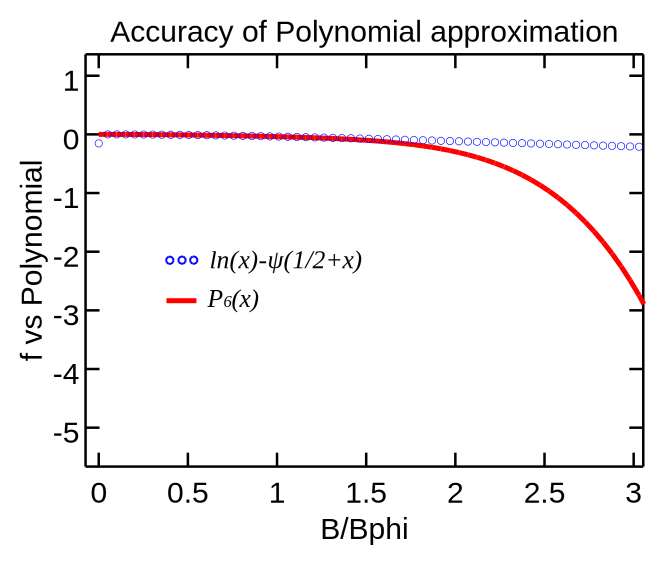
\includegraphics[scale=0.5]{fVsPoly}
	 \caption{Comparison of $f(B)$ with the polynomial approximation of the 6th degree. At very low fields the truncated Hikami-Larkin-Nagaoka function $\ln(x)-\psi\left( 1/2+x\right)$ looks like parabola.}
    \label{fig:fVsPoly}
\end{figure}
It must be noted that polynomial approximation fails miserably for $B\ge B_\epsilon$. For the fields $B\gg B_\epsilon$ the conductance increases logarithmically (see also HLN paper, Eq.~(19)):
\begin{equation}
	\sigma(B) = \sigma(0) -\frac{\alpha e^2}{2\pi^2\hbar}\ln\frac{B}{B_\epsilon}
\end{equation}
If there is any additional contribution into magnetoconductance, like normal quadratic, then it will most likely dominate the logarithmic term.

In summary, the validity of the truncated expression for the conductance
\begin{equation}
	\sigma(B) = \sigma(0) -\frac{\alpha e^2}{2\pi^2\hbar}\left[\ln\left(\frac{B_\epsilon}{B}\right) - \psi\left(\frac{1}{2}+\frac{B_\epsilon}{B}\right)\right]
\end{equation}
requires that the total scattering rate $\tau$ is large enough for the condition $1/a\tau \gg 1$ to be satisfied. From the definition of $\tau$ it follows that to apply the truncated expression we need
\begin{equation}
	\displaystyle{\frac{1}{a\tau^z_{SO}}+\frac{2}{a\tau^x_{SO}}+\frac{1}{a\tau^z_{S}}+\frac{2}{a\tau^x_{S}}+\frac{1}{a\tau_{\epsilon}}}\gg 1.
\end{equation}

If the spin-orbit interaction is very strong (like in TIs), this requirement is satisfied due to the large values of the $\tau_{SO}$-related terms. The magnitude of $\alpha$, according to Hikami-Larkin-Nagaoka, indicates which mechanism is diminant in scattering: $\alpha = 1$ corresponds to the absence of spin-orbit and magnetic scattering; 2) $\alpha = 0$ corresponds to strong magnetic scattering; 3) $\alpha = -1/2$ corresponds to absence of magnetic scattering and strong spin-orbit interactions. 

It must be kept in mind that ``{\it In strict two dimensions, the spin-orbit interaction has only the $z$-component ($1/\tau^x_{SO} = 0,\, 1/\tau^z_{SO} \ne 0$). Then, if $1/\tau_S = 0$, the behavior of the system becomes the same as unitary case without logarithmic term}''. It means that $\alpha = 0$ may also correspond to strict two-dimensions with strong spin-orbit and without magnetic scattering!

\section{Data Fitting Strategies}
The most straightforward, although not necessarily the easiest, strategy would be to fit the experimental data
\begin{equation}
	\frac{\sigma_0 - \sigma(B)}{G_0/2\pi},\quad (G_0 = \frac{2e^2}{h}\textrm{ -- conductance quantum})
\end{equation}
with the four-parameter function
\begin{equation}
	s(B) = \psi\left(\frac{1}{2}+\frac{B_1}{B}\right)-\psi\left(\frac{1}{2}+\frac{B_2}{B}\right)+\frac{1}{2}\psi\left(\frac{1}{2}+\frac{B_3}{B}\right)-\frac{1}{2}\psi\left(\frac{1}{2}+\frac{B_4}{B}\right).
\end{equation}
The number of independent parameters is actually three (3) since there is a relation between $B_1,\, B_2,\,B_3$, and $B_4$ such that the condition $s(0) = 0$ is satisfied. Indeed, considering that $\psi(1/2+x) \approx \ln(x)$ for large $x$ (small fields) we have
\begin{equation}
	s(0) = \ln\left(\frac{B_1}{B}\right)-\ln\left(\frac{B_2}{B}\right)+\frac{1}{2}\ln\left(\frac{B_3}{B}\right)-\frac{1}{2}\ln\left(\frac{B_4}{B}\right) = \frac{1}{2}\ln\frac{B_1^2B_3}{B_2^2B_4} = 0
\end{equation}
so
\begin{equation}
	\frac{B_1^2B_3}{B_2^2B_4} = 1\quad\rightarrow\quad B_4 = B_3\left(\frac{B_1}{B_2}\right)^2.
\end{equation}

									
\end{document}
